%% abtex2-modelo-artigo.tex, v-1.9.6 laurocesar
%% Copyright 2012-2016 by abnTeX2 group at http://www.abntex.net.br/ 
%%
%% This work may be distributed and/or modified under the
%% conditions of the LaTeX Project Public License, either version 1.3
%% of this license or (at your option) any later version.
%% The latest version of this license is in
%%   http://www.latex-project.org/lppl.txt
%% and version 1.3 or later is part of all distributions of LaTeX
%% version 2005/12/01 or later.
%%
%% This work has the LPPL maintenance status `maintained'.
%% 
%% The Current Maintainer of this work is the abnTeX2 team, led
%% by Lauro César Araujo. Further information are available on 
%% http://www.abntex.net.br/
%%
%% This work consists of the files abntex2-modelo-artigo.tex and
%% abntex2-modelo-references.bib
%%

% ------------------------------------------------------------------------
% ------------------------------------------------------------------------
% abnTeX2: Modelo de Artigo Acadêmico em conformidade com
% ABNT NBR 6022:2003: Informação e documentação - Artigo em publicação 
% periódica científica impressa - Apresentação
% ------------------------------------------------------------------------
% ------------------------------------------------------------------------

\documentclass[
	% -- opções da classe memoir --
	article,			% indica que é um artigo acadêmico
	11pt,				% tamanho da fonte
	oneside,			% para impressão apenas no recto. Oposto a twoside
	a4paper,			% tamanho do papel. 
	% -- opções da classe abntex2 --
	%chapter=TITLE,		% títulos de capítulos convertidos em letras maiúsculas
	%section=TITLE,		% títulos de seções convertidos em letras maiúsculas
	%subsection=TITLE,	% títulos de subseções convertidos em letras maiúsculas
	%subsubsection=TITLE % títulos de subsubseções convertidos em letras maiúsculas
	% -- opções do pacote babel --
	english,			% idioma adicional para hifenização
	brazil,				% o último idioma é o principal do documento
	sumario=tradicional
	]{abntex2}


% ---
% PACOTES
% ---

% ---
% Pacotes fundamentais 
% ---
\usepackage{lmodern}			% Usa a fonte Latin Modern
\usepackage[T1]{fontenc}		% Selecao de codigos de fonte.
\usepackage[utf8]{inputenc}		% Codificacao do documento (conversão automática dos acentos)
\usepackage{indentfirst}		% Indenta o primeiro parágrafo de cada seção.
\usepackage{color}				% Controle das cores
\usepackage{graphicx}			% Inclusão de gráficos
\usepackage{microtype} 			% para melhorias de justificação
\usepackage{amsmath}
% ---
		
% ---
% Pacotes adicionais, usados apenas no âmbito do Modelo Canônico do abnteX2
% ---
\usepackage{lipsum}				% para geração de dummy text
% ---
		
% ---
% Pacotes de citações
% ---
\usepackage[brazilian,hyperpageref]{backref}	 % Paginas com as citações na bibl
\usepackage[alf]{abntex2cite}	% Citações padrão ABNT
% ---

% ---
% Configurações do pacote backref
% Usado sem a opção hyperpageref de backref
\renewcommand{\backrefpagesname}{Citado na(s) página(s):~}
% Texto padrão antes do número das páginas
\renewcommand{\backref}{}
% Define os textos da citação
\renewcommand*{\backrefalt}[4]{
	\ifcase #1 %
		Nenhuma citação no texto.%
	\or
		Citado na página #2.%
	\else
		Citado #1 vezes nas páginas #2.%
	\fi}%
% ---

% ---
% Informações de dados para CAPA e FOLHA DE ROSTO
% ---
\titulo{Modelo Canônico de\\ Artigo científico com \abnTeX}
\autor{Equipe \abnTeX\thanks{\url{http://www.abntex.net.br/}} \and Lauro
César
Araujo\thanks{laurocesar@laurocesar.com}}
\local{Brasil}
\data{2015, v-1.9.6}
% ---

% ---
% Configurações de aparência do PDF final

% alterando o aspecto da cor azul
\definecolor{blue}{RGB}{41,5,195}

% informações do PDF
\makeatletter
\hypersetup{
     	%pagebackref=true,
		pdftitle={\@title}, 
		pdfauthor={\@author},
    	pdfsubject={Modelo de artigo científico com abnTeX2},
	    pdfcreator={LaTeX with abnTeX2},
		pdfkeywords={abnt}{latex}{abntex}{abntex2}{atigo científico}, 
		colorlinks=true,       		% false: boxed links; true: colored links
    	linkcolor=blue,          	% color of internal links
    	citecolor=blue,        		% color of links to bibliography
    	filecolor=magenta,      		% color of file links
		urlcolor=blue,
		bookmarksdepth=4
}
\makeatother
% --- 

% ---
% compila o indice
% ---
\makeindex
% ---

% ---
% Altera as margens padrões
% ---
\setlrmarginsandblock{3cm}{3cm}{*}
\setulmarginsandblock{3cm}{3cm}{*}
\checkandfixthelayout
% ---

% --- 
% Espaçamentos entre linhas e parágrafos 
% --- 

% O tamanho do parágrafo é dado por:
\setlength{\parindent}{1.3cm}

% Controle do espaçamento entre um parágrafo e outro:
\setlength{\parskip}{0.2cm}  % tente também \onelineskip

% Espaçamento simples
\SingleSpacing

% ----
% Início do documento
% ----
\begin{document}

% Seleciona o idioma do documento (conforme pacotes do babel)
%\selectlanguage{english}
\selectlanguage{brazil}

% Retira espaço extra obsoleto entre as frases.
\frenchspacing 

% ----------------------------------------------------------
% ELEMENTOS PRÉ-TEXTUAIS
% ----------------------------------------------------------

%---
%
% Se desejar escrever o artigo em duas colunas, descomente a linha abaixo
% e a linha com o texto ``FIM DE ARTIGO EM DUAS COLUNAS''.
% \twocolumn[    		% INICIO DE ARTIGO EM DUAS COLUNAS
%
%---
% página de titulo
\maketitle

% resumo em português
\begin{resumoumacoluna}
Neste trabalho, são apresentados problemas de modelagem matemática sugeridos pelo livro Equações Diferenciais Ordinárias, do autor Dennis G. Zill. O processo de modelagem é algo que pode ser bastante interdisciplinar, visto que, são utilizados conceitos das mais diversas áreas de estudo e conhecimento para estruturação e resolução do problema.
 
 \vspace{\onelineskip}
 
 \noindent
 \textbf{Palavras-chave}: latex. abntex. editoração de texto.
\end{resumoumacoluna}

\textual

\section*{Modelagem matemática: o que é?}
\addcontentsline{toc}{section}{Modelagem matemática: o que é?}

A modelagem matemática é uma área de conhecimento que estuda a simulação de sistemas e situações reais, com o objetivo de prever como deve será o comportamento e o resultado dos mesmos. Abrange várias áreas de estudo, como física, biologia, engenharia, química, entre outros.

Umas das formas que continuam sendo muito utilizadas para a modelagem desses problemas, é a partir das equações diferenciais.

\section{Desenvolvimento}
\subsection{Questões propostas}
\subsubsection{Problema 1.1.24}
Suponha que um buraco tenha sido feito através do centro da Terra, atravessando-a de ponta a ponta, e uma bola de boliche com massa $m$ seja jogada no buraco, conforme mostra a figura abaixo. Construa um modelo matemático que descreve o movimento da bola. Em um dado instante $t$, seja $r$ a distância do centro da Terra até a massa $m$, $M$ a massa da Terra, $M_{r}$ a massa da parte da Terra dentro de uma esfera de raio $r$ e $\delta$, a densidade constante da Terra. \\

\centerline{\begin{minipage}[c]{\textwidth}
		\centering
		\noindent
		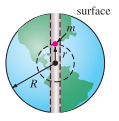
\includegraphics[width=0.3\textwidth]{imagem.png}
		\label{}
\end{minipage}}
		\subsubsubsection{Problematização}
		Devemos construir um modelo matemático que relacione o movimento que a bola de boliche, em queda, em um instante t á uma distância r do centro da terra.
		
		\subsubsubsection{Dados}
		\begin{center}
			\noindent $m= $\textit{ massa da bola de boliche\\}
			\noindent $M=$\textit{ massa da Terra\\}
			\noindent $r=$\textit{ distância entre a bola e o centro da Terra\\}
			\noindent $M_{r}=$\textit{ massa dentro do raio\\}
			\noindent $R=$\textit{ raio da Terra\\}
			\noindent $\delta = $\textit{ densidade constante da Terra\\}
		\end{center}

		
		\subsubsubsection{Construção do modelo}
		Partindo da segunda lei de Newton, a qual afirma que a força resultante que atua sobre um corpo é proporcional ao produto da massa pela aceleração por ele adquirida. Logo:
		\begin{equation}\label{eq1}
		F_{r} = m \cdot a
		\end{equation}
		É conhecido também, que a aceleração pode ser obtida a partir da derivada da velocidade em relação a um instante t, que por sua vez é a derivada de um espaço r em relação a um instante t. Assim, podemos definir a aceleração de um corpo, como a derivada de segunda ordem de r em relação a t:\\
		
		\begin{equation}\label{eq2}
		a = \frac{d^{2}r}{dt^{2}}
		\end{equation}
		
		\noindent Aplicando (\ref{eq2}) em (\ref{eq1}), obtém-se:
		\begin{equation}\label{eqf}
		F_{R} = m \cdot \frac{d^{2}r}{dt^{2}}
		\end{equation}
		
		\noindent Para obtermos as respectivas massas, podemos valer-nos da seguinte característica intrínseca dos sólidos:
\begin{equation*}
	d= \frac{M}{V}
\end{equation*}

\noindent Onde $d$ é a densidade do sólido, $M$ a massa e $V$ o volume do mesmo.
Logo:
\begin{equation*}
M = d \cdot V
\end{equation*}
\noindent Como os objetos em questão possuem formato esférico, teremos:
\begin{equation*}
V = \frac{4\pi R^{3}}{3}
\end{equation*}

\noindent Assim:
\begin{equation}\label{eq3}
M = \frac{4\pi R^{3}}{3} \cdot \delta \rightarrow M_{r} = \frac{4\pi R^{3}}{3} \cdot \delta
\end{equation}

\noindent Para fins de simplificação, podemos fazer o seguinte:
\begin{equation}\label{eq4}
M = \frac{4\pi R^{3}}{3} \cdot \delta \rightarrow 4\pi \delta = \frac{3M}{R^{3}}
\end{equation}

\noindent Aplicando \eqref{eq4} em \eqref{eq3}, obteremos:
\begin{equation*}
M_{r}= \frac{M \cdot r^{3}}{R^{3}}
\end{equation*}

Baseado na lei de gravitação universal, formulada por Isaac Newton, podemos afirmar que força de atração gravitacional entre dois corpos é diretamente proporcional a massa dos corpos em questão e inversamente proporcional ao quadrado da distância entre os dois corpos.
\begin{equation*}
F_{G} = G \cdot \frac{m_{1} \cdot m_{2}}{r^{2}}
\end{equation*}

\noindent A força gravitacional entre $m$ e $M_{r}$, é dada então por:
\begin{equation*}
F_{G} = G \cdot \frac{m \cdot \frac{M \cdot r^{3}}{R^{3}}}{r^{2}} \rightarrow F_{G} = G \cdot \frac{m \cdot M \cdot r^{3}}{R^{3} \cdot r^{2}}
\end{equation*}

\begin{equation}\label{eq5}
F_{G} = G \cdot \frac{m \cdot M \cdot r}{R^{3}}
\end{equation}

\noindent Agora, pode-se fazer uma relação de igualdade entre as forças \eqref{eqf} e \eqref{eq5}:
\begin{equation*}
F_{R} = F_{G}
\end{equation*}
\begin{equation*}
m \cdot \frac{d^{2}r}{dt^{2}} = G \cdot \frac{m \cdot M \cdot r}{R^{3}}
\end{equation*}
\begin{equation}\label{eq6}
\frac{d^{2}r}{dt^{2}} = G \cdot \frac{M \cdot r}{R^{3}}
\end{equation}

\textbf{A \autoref{eq6} é o modelo matemático que relaciona as grandezas necessárias, a uma distância $r$ e um instante $t$.}
\end{document}
